\section{Example: Space Resection}
A space resection is used to calculate the camera pose, or exterior orientation, using correspondences between pixel coordinates and world coordinates, as well as a known camera interior orientation.

\vspace{.5cm}\noindent
Tait-Bryan Rotation Matrix Convention (ZYX)
\[R = 
\begin{bmatrix}
	r_{11} & r_{12} & r_{13} \\
	r_{21} & r_{22} & r_{23} \\
	r_{31} & r_{32} & r_{33} \\
\end{bmatrix}
=
\begin{bmatrix}[1.5]
	\cos(\kappa)\cos(\phi) &
	\cos(\phi)\sin(\kappa) &
	-\sin(\phi) \\
	\cos(\kappa)\sin(\omega)\sin(\phi) - \cos(\omega)\sin(\kappa) &
	\cos(\kappa)\cos(\omega) + \sin(\kappa)\sin(\omega)\sin(\phi) &
	\cos(\phi)\sin(\omega) \\
	\sin(\kappa)\sin(\omega) + \cos(\kappa)\cos(\omega)\sin(\phi) &
	\cos(\omega)\sin(\kappa)\sin(\phi) - \cos(\kappa)\sin(\omega) &
	\cos(\omega)\cos(\phi) \\
\end{bmatrix}
\]
\subsection{Computer Vision Nomenclature Equations}
\begin{align*}
s &= \text{Z Distance (perpendicular to camera focal plane) from Camera to XYZ world coordinate} \\
u &= \text{Camera x pixel} \\
v &= \text{Camera y pixel} \\
K & = \text{Camera Interior Orientation} \\
f_x &= \text{x focal length in pixels} \\
f_y &= \text{y focal length in pixels} \\
c_x &= \text{x principal point} \\
c_y &= \text{y principal point} \\
\begin{bmatrix} RT \end{bmatrix} &= \text{Camera Exterior Orientation} \\
\begin{bmatrix}	X_w \\ Y_w \\ Z_w \\ 1 \end{bmatrix} &= \text{Homogeneous World Coordinate}
\end{align*}
\begin{align*}
s\times
\begin{bmatrix}	u \\ v \\ 1 \end{bmatrix} 
&=
K
\begin{bmatrix} RT \end{bmatrix}
\begin{bmatrix}	X_w \\ Y_w \\ Z_w \\ 1 \end{bmatrix} \\
s\times
\begin{bmatrix}	u \\ v \\ 1 \end{bmatrix} 
&= \begin{bmatrix}
f_x & 0 & c_x \\
0 & f_y & c_y \\
0 & 0 & 1 
\end{bmatrix}
\begin{bmatrix}
r_{11} & r_{12} & r_{13} & T_x\\
r_{21} & r_{22} & r_{23} & T_y\\
r_{31} & r_{32} & r_{33} & T_z
\end{bmatrix}
\begin{bmatrix}	X_w \\ Y_w \\ Z_w \\ 1 \end{bmatrix}
\end{align*}

$(\omega,\phi,\kappa,T_x,T_y,T_z,s)$ = Space Resection Unknowns *Note that s is related to the rotation, so 
\clearpage
\subsection{Photogrammetry Nomenclature: "Collinearity Equations"}
The photogrammetry nomenclature is slightly different, but as you can see, the equations are the same.
\begin{figure}[H]
	\centering
	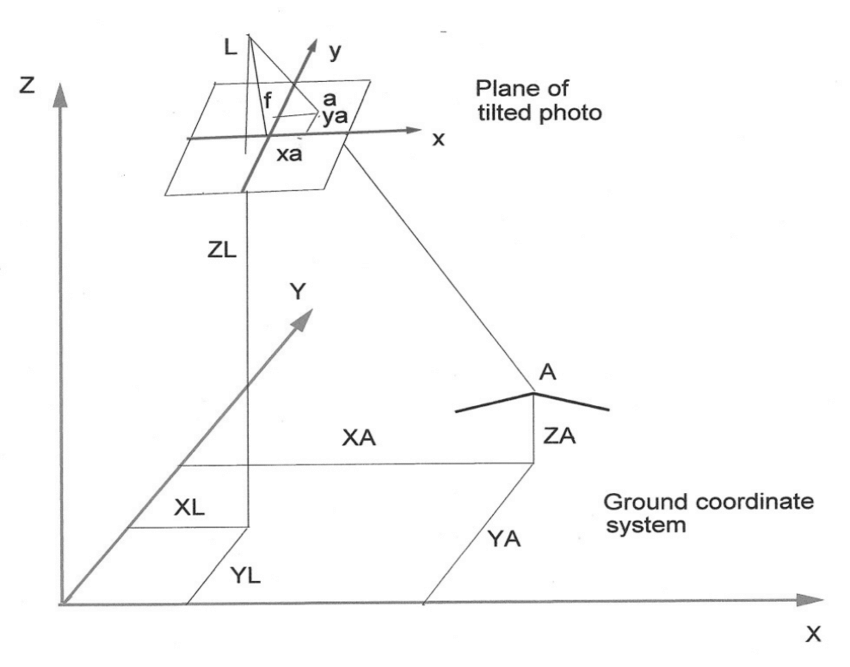
\includegraphics[height = 3in]{collinearity}
\end{figure}
\begin{align*}
	X_A,Y_A,Z_A &= \text{World Coordinates} \\
	X_L,Y_L,Z_L &= \text{Camera Position in World Coordinates} 
\end{align*}
\begin{align*}
s\times
\begin{bmatrix}	x \\ y \\ 1 \end{bmatrix} 
&= \begin{bmatrix}
f_x & 0 & c_x \\
0 & f_y & c_y \\
0 & 0 & 1 
\end{bmatrix}
\begin{bmatrix}
r_{11} & r_{12} & r_{13}\\
r_{21} & r_{22} & r_{23}\\
r_{31} & r_{32} & r_{33}
\end{bmatrix}
\begin{bmatrix}	X_A-X_L \\ Y_A-Y_L \\ Z_A-Z_L \end{bmatrix}
\end{align*}
Collinearity Equations: \todo{above equation is wrong compared to collinearity...}
\begin{align*}
x &= x_0 - f\left[\dfrac{r_{11}(X_A-X_L) + r_{12}(Y_A-Y_L) + r_{13}(Z_A-Z_L)}{r_{31}(X_A-X_L) + r_{32}(Y_A-Y_L) + r_{33}(Z_A-Z_L)}\right] \\
y &= y_0 - f\left[\dfrac{r_{21}(X_A-X_L) + r_{22}(Y_A-Y_L) + r_{23}(Z_A-Z_L)}{r_{31}(X_A-X_L) + r_{32}(Y_A-Y_L) + r_{33}(Z_A-Z_L)}\right]
\end{align*}
$(\omega,\phi,\kappa,X_L,Y_L,Z_L)$ = Space Resection Unknowns

There are 6 unknowns which must be solved to determine the camera exterior orientation. For every 3D Coordinate with a corresponding pixel coordinate, there are 2 observation.  Therefore, for an over-constrained solution, you need at least 4 world coordinates.  *note: these points 